\documentclass[a4paper]{article}
\usepackage[numbers,super,comma]{natbib}
\bibliographystyle{unsrt}
\usepackage{amsmath}
\usepackage{float}
\usepackage{subfig}
\usepackage{geometry}
\geometry{left=3cm,right=3cm}
\usepackage{titlesec}
\usepackage{titletoc}
\usepackage{booktabs}
\usepackage{hyperref}
\usepackage{tcolorbox}
\tcbuselibrary{most}
\definecolor{light-gray}{gray}{0.92}
\definecolor{dark-gray}{gray}{0.32}
\newcommand{\HRule}{\rule{\linewidth}{0.5mm}}
\usepackage{hyperref}

\usepackage{listings}
\usepackage{xcolor}
\lstset{
    columns=fixed,       
    numbers=left,                                        % 在左侧显示行号
    frame=none,                                          % 不显示背景边框
    backgroundcolor=\color[RGB]{255,255,255},            % 设定背景颜色
    keywordstyle=\color[RGB]{40,40,255},                 % 设定关键字颜色
    numberstyle=\footnotesize\color{darkgray},           % 设定行号格式
    commentstyle=\it\color[RGB]{0,96,96},                % 设置代码注释的格式
    stringstyle=\rmfamily\slshape\color[RGB]{128,0,0},   % 设置字符串格式
    showstringspaces=false,                              % 不显示字符串中的空格
    language=python,                                        % 设置语言
}

\begin{document}
\newtheorem{assumption}{Assumption}
\begin{center}
\LARGE{\textbf{Causes and Solutions to U.S. Opioid Crisis\\}}
\vspace{6mm}
\normalsize{Shuo Liu$^1$, Rui Xi$^1$, Rui Yang$^1$, Yuqi Wu$^1$}\\
\vspace{2mm}
\small{SDCS, SYSU}\\
\end{center}

\begin{figure}[h]
	\centering  
	
\includegraphics[width=0.3\linewidth]{OpioidCrisis/sysu.png} 
\end{figure}

%% === 0. Abstract === %%
\noindent \HRule
\renewcommand{\baselinestretch}{1.8}
\begin{center}
    \textbf{\large{Summary}}
\end{center}
With the opioid crisis becoming a national concern, the federal government is struggling to figure out how to respond. Why does it happen? How does it evolve? And what can we do to deal with it? Here, we proposed model \texttt{OCEAN} and its enhancement \texttt{D-OCEAN} to delve into the evolution of opioids.

We first get the growth pattern of drug reported quantity through a large number of data analysis and case studies. We observe that: \textbf{(a)} A county owns a similar growth pattern with its nearby.  \textbf{(b)} Linear growth patterns can be found in counties who are isolated by similarity with the surrounding. Based on such observations, we assume that the increase in drug reports is made up of two main components: \textbf{intrinsic increment} and \textbf{extrinsic influence} from nearby counties. Then we defined a cellular automata to simulate evolution of opioid cases for all counties. Reverse evolving, origin of a specific opioid can be traced. Forward evolving, prediction is made for each location.

After that, we further consider the \textbf{socio-economic factors} and modify our model. By computing the Pearson correlation coefficient between drug reported quantity and the socio-economic factors, we find some important \textbf{demographic features} which are highly related to opioid use. \textbf{K-means} algorithm is then applied to group data into several groups, each of which represents a typical type. Our results have been reversely verified to ensure the accuracy of similarity analysis. Taking the idea of simulate anneal, we add a new update rule to make intrinsic factor more considerate. As proved by comparative experiments, enhanced model possesses a higher robustness and more accurate predict results.

Base on our works above, we present some strategies for countering the opioid crisis. We validate that such strategies can really improve the opioid epidemic situation and sensitivity analysis shows the utility of each strategy. 

In conclusion, we employ a cellular automata for simulating the evolution patterns of opioids in \textbf{Task I}. We enhanced our model in \textbf{Task II} by introducing some socio-economic factors, taking account of demographic heterogeneity in each state. Finally, corresponding solutions were put forward, according to the analysis of our models.


\noindent \HRule
\renewcommand{\baselinestretch}{1.0}
\clearpage
\renewcommand{\baselinestretch}{0.5}
\tableofcontents
\renewcommand{\baselinestretch}{1.0}
\clearpage

\section{Problems}

\subsection{Background}

The United States is experiencing a national crisis regarding the use of synthetic and non- synthetic opioids, either for the treatment and management of pain (legal, prescription use) or for recreational purposes (illegal, non-prescription use). Federal organizations such as the Centers for Disease Control (CDC) are struggling to “save lives and prevent negative health effects of this epidemic, such as opioid use disorder, hepatitis, and HIV infections, and neonatal abstinence syndrome.” Simply enforcing existing laws is a complex challenge for the Federal Bureau of Investigation (FBI), and the U.S. Drug Enforcement Administration (DEA), among others.

There are implications for important sectors of the U.S. economy as well. For example, if the opioid crisis spreads to all cross-sections of the U.S. population (including the college-educated and those with advanced degrees), businesses requiring precision labor skills, high technology component assembly, and sensitive trust or security relationships with clients and customers might have difficulty filling these positions. Further, if the percentage of people with opioid addiction increases within the elderly, health care costs and assisted living facility staffing will also be affected.

The DEA/National Forensic Laboratory Information System (NFLIS), as part of the Drug Enforcement Administration's (DEA) Office of Diversion Control, publishes a data-heavy annual report addressing "drug identification results and associated information from drug cases analyzed by federal, state, and local forensic laboratories." The database within NFLIS includes data from crime laboratories that handle over 88\% of the nation's estimated 1.2 million annual state and local drug cases. For this problem, we focus on the individual counties located in five (5) U.S. states: Ohio, Kentucky, West Virginia, Virginia, and Tennessee. In the U.S., a county is the next lower level of government below each state that has taxation authority.

\subsection{Dataset}

We collect and download several datasets from DEA and other American drug administration. The first file (MCM\_NFLIS\_Data.xlsx) contains drug identification counts in years 2010-2017 for narcotic analgesics (synthetic opioids) and heroin in each of the counties from these five states as reported to the DEA by crime laboratories throughout each state. A drug identification occurs when evidence is submitted to crime laboratories by law enforcement agencies as part of a criminal investigation and the laboratory’s forensic scientists test the evidence. Typically, when law enforcement organizations submit these samples, they provide location data (county) with their incident reports. When evidence is submitted to a crime laboratory and this location data is not provided, the crime laboratory uses the location of the city/county/state investigating law enforcement organization that submitted the case. For the purposes of this problem, we can assume that the county location data are correct as provided.

The additional seven (7) files are zipped folders containing extracts from the U.S. Census Bureau that represent a common set of socio-economic factors collected for the counties of these five states during each of the years 2010-2016 (ACS\_xx\_5YR\_DP02.zip). \textit{(Note: The same data were not available for 2017.)} All of the datasets we used have been push on the transfer gate, you can download them via \href{https://github.com/LovelyBuggies/Python_2019MCM_OpioidCrisis/raw/master/Problems/dataset.zip}{this link}.

%% === 1. Introduction === %%

\section{Introduction} 

With the nationwide opioid epidemic, making good use of them and preventing their negative health effects have become one of the urgent missions for the U.S. Centers of Disease Control (CDC). \cite{CDC} In addition to some synthetic opioids used for medical anesthesia, large quantities of addictive heroin and other non-synthetic opioids have entered the market, seriously jeopardizing the health of American citizens and bringing huge economic and social pressure to the U.S. government. \cite{opioidrelation} Despite legislative, law enforcement, and judicial efforts, the trend in opioid abuse does not appear to have abated so far. \cite{law2018, DEA2018} As the number of illnesses and deaths increases, the opioid crisis is shaping up to be a catastrophe for American society. \cite{opioidcrsis}

As the opioid crisis has been greatly concerned, the National Forensic Laboratory Information System (DEA/NFLIS) collects fairly comprehensive data from crime laboratories around the country, hoping to find effective coping strategies by analyzing it. Here, we are expected to help NFLIS identify the causes of the opioid crisis and to propose practical solutions. Specifically, we mainly focus on individual counties located in five U.S. states (VA, OH, PA, WV, KY), and set the following goals:

\begin{itemize} 
\item Describe spread and characteristics of opioid incidents.
\item Speculate on the origins of opioids and predict their future.
\item Give analysis of the correlation between opioid use and socio-economic factors.
\item Find possible strategies to deal with the opioid crisis and analyze their feasibility.
\end{itemize}

Many existing models have shed lights on the pattern of opiate addiction transmission. Early in 1997, D.R. Mackintosh, G.T. Stewart proposed an exponential model to illustrate how the use of heroin spreads in epidemic fashion.\cite{model1979} Based on the principles of epidemiology, Emma White and Catherine Comiskey present an ODE model of opiate addiction in 2007.\cite{model2007} G.P. Samanta modified the White and Comiskey heroin epidemic model into a non-autonomous heroin epidemic model with distributed time delay.\cite{model2011} However, to our best knowledge, most of the existing models are small-range transmission models based on epidemiological principles, no model uses finite automata to simulate large-scale drug transmission. In addition, these models only mention non-prescriptive opioids like heroin, but prescription drugs may have very different patterns in transmission to some extent. More importantly, given the heterogeneity of states, many studies inspire us to take demographic structure into account. \cite{hetro, demogen2001}

\begin{figure}[h]
	\centering  
	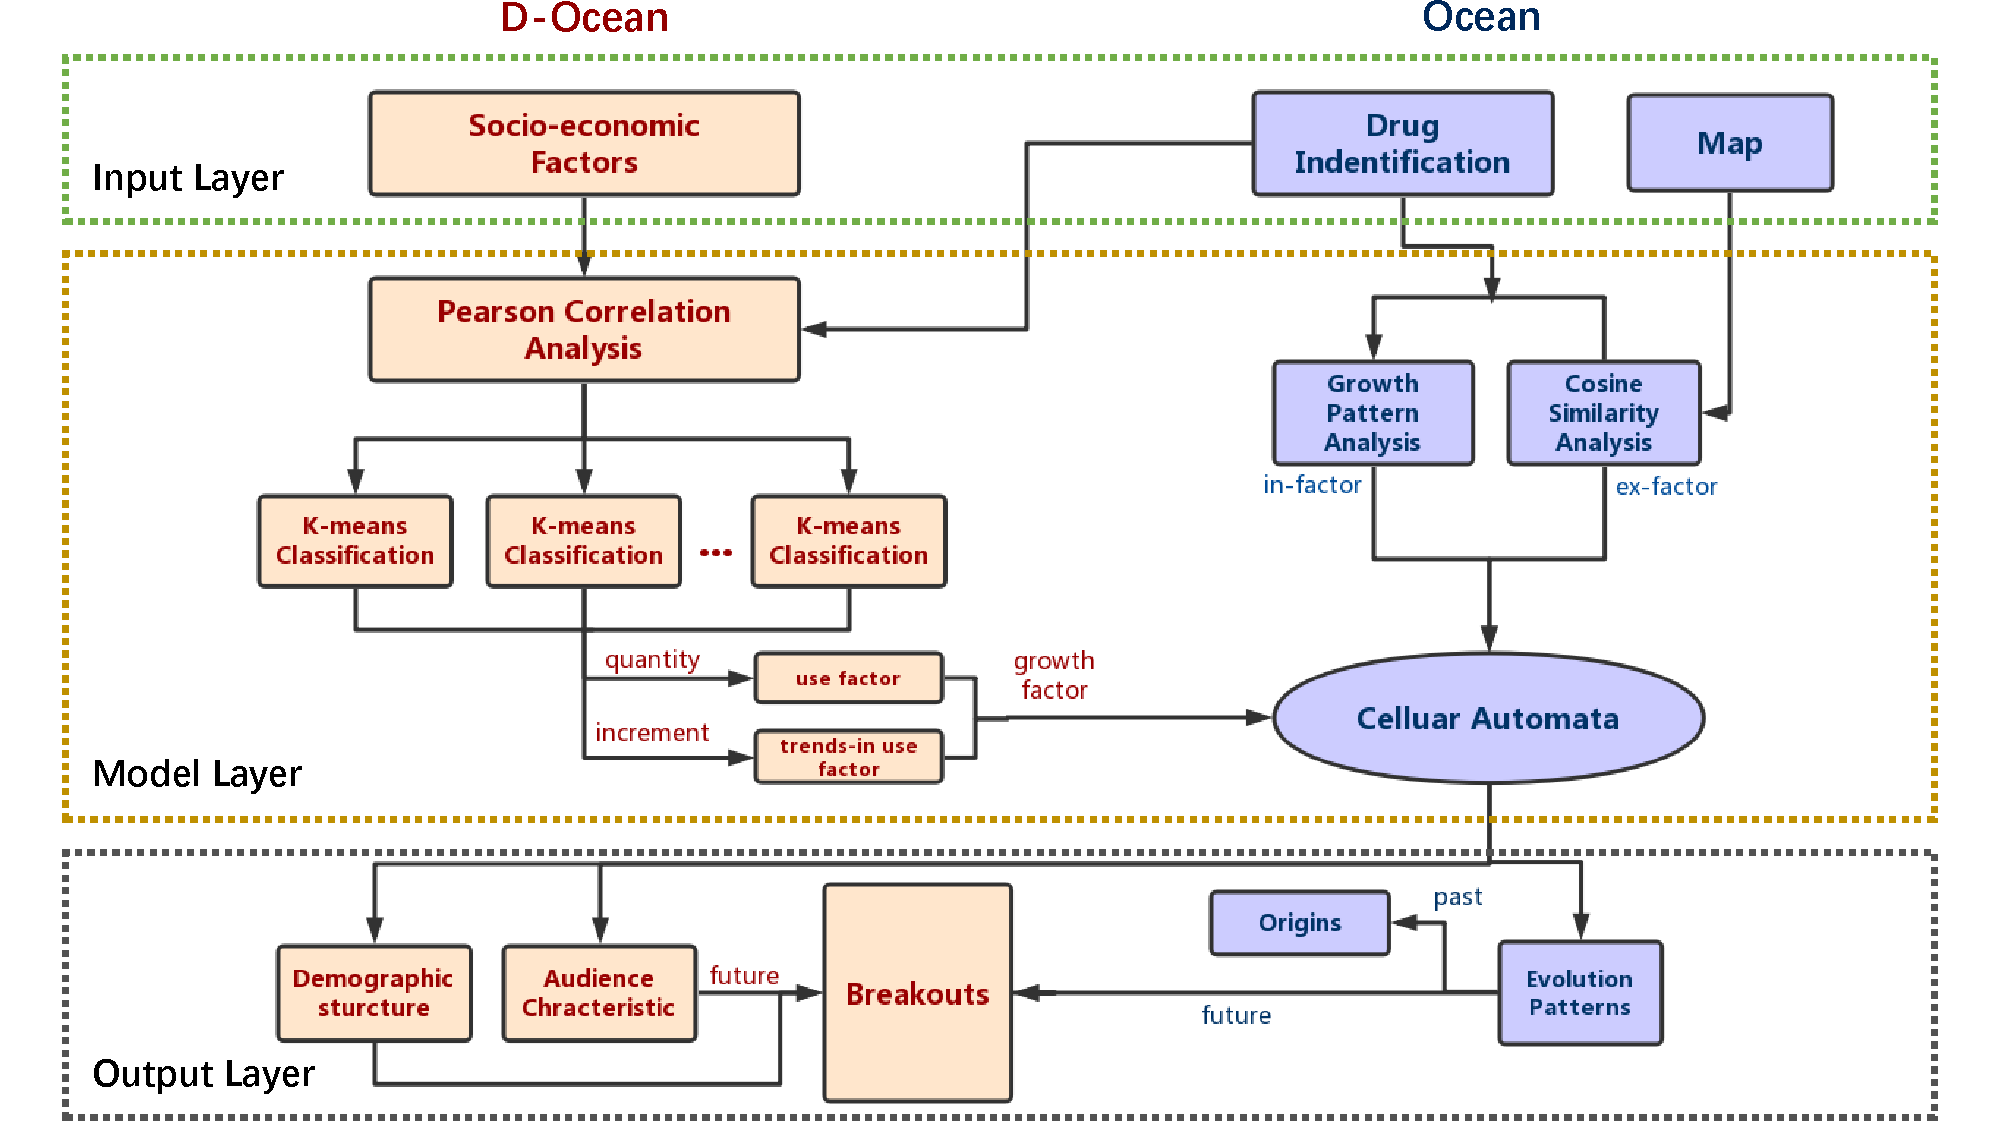
\includegraphics[width=1.0\linewidth]{OpioidCrisis/figures/Model.pdf} 
	\caption{Framework of our model: \texttt{OCEAN} and \texttt{D-OCEAN}} 
	\label{fig:model}
\end{figure}

In this work, we proposed a novel model called \texttt{OCEAN} and its enhancement \texttt{D-OCEAN} to cope with the opioid crisis. The framework of \texttt{OCEAN} and \texttt{D-OCEAN} is shown in \textbf{Figure} \ref{fig:model}.

Our framework in \textbf{Figure} \ref{fig:model} has the following attributes:

\begin{itemize}
    \item \textbf{\large{2} \normalsize Models:} \texttt{OCEAN} and \texttt{D-OCEAN} are involved in our framework to solving problem in \textbf{Task I} and \textbf{Task II} respectively.
    \item \textbf{\large{3} \normalsize Layers:} Socio-economic factors, drug identification as well as download map are input from \textsf{input layer} to \textsf{model layer} for modeling, and then generate the final results. 
    \item \textbf{\large{4} \normalsize Update Rules:} Our models follow 4 update rules to estimate the drug reported quantity and increment in the next year.
    \item \textbf{\large{5} \normalsize Techniques:} We mainly apply 5 techniques to accomplish our framework: cosine similarity analysis, Pearson similarity analysis, cellular automata simulation, K-means algorithm and simulate anneal.
\end{itemize}
\vspace{4pt}


%% === 2. Assumptions  Definitions === %%
\section{Assumptions and Definitions}

%% === 2.1 General Assumptions
\subsection{General Assumptions}

\vspace{4pt}
\begin{assumption}
  \textit{The effect of irresistible factors like warfare and nature disaster will not be taken into consideration in this problem.}
\end{assumption}
Upheaval of situations cause by inevitable cases are supposed to be neglected for difficulty of prediction.

\vspace{8pt}
\begin{assumption}
  \textit{The provided data is accurate and reliable so that we can obtain correct information from it.}
\end{assumption}
The accuracy of the data is the cornerstone of the experiment.

\vspace{8pt}
\begin{assumption}
  \textit{There is drug flow from county to county.}
\end{assumption}
In real life, proximity facilitates the spread of drugs.

\vspace{8pt}
\begin{assumption}
  \textit{There is a correlation between drug cases and demographics features.}
\end{assumption}
The heterogeneity of county population is an important cause of event deviation.

%% === 2.2 General Definitions === %%
\subsection{General Definitions}

\begin{itemize}
  \item \textbf{Drug reports/opioid cases:} reported opioid incidents in counties. We mainly focus on two aspects of them: the quantity and the increment.
  \vspace{4pt}
  
  \item \textbf{Evolution:} sum of all forms of motion in a given space-time. In this situation, evolution represents spread and characteristics of opioid incidents.
  \vspace{4pt}
  
  \item \textbf{Opioid-increment island:} county whose incremental trend is not similar to all its surrounding counties. The evolution of opioid-increment islands is relatively isolated.
  \vspace{4pt}
  
  \item \textbf{Cellular automaton:} local grid dynamics model with discrete time, space and state, which are able to simulate spatio-temporal evolution of complex systems.\cite{cellularA}
  \vspace{4pt}
  
  \item \textbf{Demographic features:} socio-economic features (e.g. fertility, educational attainment, marital status) of the population. Note that demographic features can be directly extract from data given.
  \vspace{4pt}
  
  \item \textbf{Significant characteristics:} some prominent characteristics that mined from demographic statistics, e.g. poor family relations, overseas, educational level etc. Significant characteristics are not intuitive information and can only be obtained by data mining.
  \vspace{4pt}
  
  \item \textbf{K-means algorithm:} method which builds $k$ classes with minimal distance among the sample observations. \cite{kmeans}
  \vspace{4pt}
  
  \item \textbf{Cluster score:} correlation between the drug reported quantity and a particular significant characteristics. A cluster with high score is more likely to have a strong relation with opioid cases.
  \vspace{4pt}
  
  \item \textbf{Use factor:} factor measuring the number of crowds who have the highly correlated demographic features. When a county has a large use factor, it may be closely linked to the drug incidents.
  \vspace{4pt}
  
  \item \textbf{Trends-in-use factor:} factor reflecting the level of outbreak vitality. When a county has a large trends-in-use factor, it may have a tremendous explosive potential with respect to certain opioids.
  \vspace{4pt}
  
\end{itemize}

%% === 3. OCEAN Model Design === %%

\section{\textbf{Task I}: Model Evolution of Opioid Cases}

%% === 3.1 Model Description === %%
\subsection{Model Description}

In this part, we build a grid dynamics model named \textbf{National Opioid-cases Evolution Cellular Automaton} (\texttt{OCEAN}), which serves to describe the spread and characteristics of opioid cases in five U.S. states. The objective of this part of model is to trace the origin of opioids and to predict potential future outbreak sites in each state.

Firstly, obtaining the geographical coordinates and distances among counties, we use \textbf{cosine similarity} formula to get the correlation of opioid cases between any two counties. A lot of hidden information is mined and put forward to make some basic assumptions. Based on these assumptions, we take advantage of a discrete, stochastic \textbf{cellular automata}, effectively simulating the evolution of reported synthetic opioid and heroin incidents.

By performing reverse evolution on cellular automata, we obtained the origin of specific opioids in each state. Moreover, results of the evolution allow us to predict when and where a particular opioid might flood. \texttt{OCEAN} will help to identify potential drug abuse in future for prevention.

%% === 3.2 Model Assumption === %%

\subsection{Model Assumption}

\vspace{4pt}
\begin{assumption}
  \textit{There are interactions between closer counties about opioid incidents within a certain range.}
\end{assumption}
By comparing the similarity of the opioid reports increment in different counties of five states, we find that some of the closest cities had similar growth patterns between 2010 and 2018. This gives us reason to believe that there may be some interactions between nearby cities.

\vspace{8pt}
\begin{assumption}
  \textit{Growth patterns of the opioid-increment islands are nearly linear.}
\end{assumption}
Opioid-increment island refers to a county where the incremental trend is not highly similar to all its surrounding cities. Through a large number of data analysis and case studies, we find that growth patterns of these opioid-increment islands are approximately linear.

\vspace{8pt}
\begin{assumption}
  \textit{Estimate of the drug reports for a county in the next year is calculated by the combination of intrinsic and extrinsic factor.}
\end{assumption}
According to the assumptions above, we put other factors on the back burner and only focus on two growth-factors, \textit{i.e.} intrinsic factor and extrinsic factor. In other words, update rules of \texttt{OCEAN} mainly take these two factors into consideration.

%% === 3.3 Mathematical Notations === %%

\subsection{Mathematical Notations}

In this part, we use the notations in \textbf{Table} \ref{tab1e33} to present the indicators in our \texttt{OCEAN}. 

\renewcommand{\baselinestretch}{1.3}
\vspace{8pt}
\begin{table}[h]
\begin{center}
\setlength{\tabcolsep}{6mm}{
\begin{tabular}{c|c}
\toprule
\textbf{Notations}& \textbf{Descriptions}\\
\hline
$t$& Year of drug reports \\
\hline
$c_n$& County $n$ in \small{VA, OH, PA, WV, KY} \\
\hline
$\mathcal{NB}$ & Nearby county collection \\
\hline
$R$, $\Delta R$& drug reported quantity and annual increment\\
\hline
$\Delta R_{in}$, $\Delta R_{ex}$ & Intrinsic and extrinsic growth quantity\\
\hline
$\hat{R}$, $\Delta \hat{R}$& Estimate of drug reported quantity and increment\\
\hline
$k_{in}$, $k_{ex}$& Weight of intrinsic and extrinsic opioid growth quantity\\
\hline
$S(c,c')$ & Similarity of opioids' growth pattern between $c$ and $c'$\\
\hline
$\alpha$, $\beta$ & Incremental parameter of intrinsic and extrinsic opioid growth \\
\bottomrule
\end{tabular}}
\caption{Mathematical Notations}
\label{tab1e33}
\end{center}
\end{table}
\renewcommand{\baselinestretch}{1.0}

%% ==== 3.3 Model Details === %%
\subsection{Model Details}

%% === 3.3.1 Problems === %%
\subsubsection*{Problems}

The description of spread and characterization of opioids can be attributed to the evolution of a complex systems. Discrete, stochastic cellular automata, having the ability to simulate the spatio-temporal evolution of complex systems, naturally becomes our first choice. 

In this problem, we are given drug identification counts $R^{(c_n,t)}$ in year 2010-2017 for narcotic analgesics and heroin in each of the counties. Our objective is to use these data to simulate the evolution of reported synthetic opioids and heroin between different counties over time. 

%% === 3.3.2 Methods === %%
\subsubsection*{Methods}

\begin{figure}[h]
	\centering  
	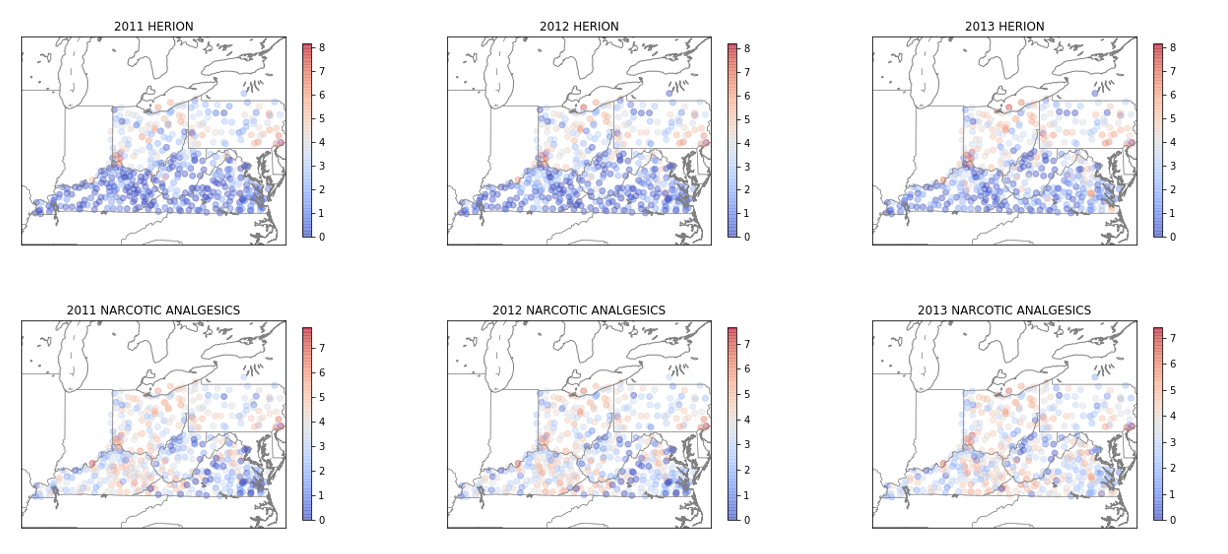
\includegraphics[width=1.0\linewidth]{OpioidCrisis/figures/overview.png} 
	\caption{Overview on the distribution of synthetic opioid and heroin.} 
	\label{fig:overview}  
\end{figure}

We first visualized the data as \textbf{Figure} \ref{fig:overview} to help to have a better overview on the synthetic opioid and heroin distribution.

Because of the our assumption that some extrinsic factors may participate in the opioid evolution, so it is necessary to consider the correlation of geographical effects. After getting the increment $\Delta R$ of drug reports in each county with the previous data, we decide to use cosine similarity to analyze the influence between counties. Specifically, the similarity of growth modes of county $c$ and county $c'$ can be expressed by the following formula.
  
\begin{equation}
    S(c,c')=\frac{\Delta \mathbf{R}^{(c)}\centerdot \Delta \mathbf{R}^{(c')}}{\|\Delta \mathbf{R}^{(c)}\|\cdot\|\Delta \mathbf{R}^{(c')}\|}
\end{equation}
\vspace{4pt}

Added inherent growth into consideration, we employ cellular automaton $A= (L,S,N,f)$ to simulate the opioid evolution of counties, where $L$ is cellular space - counties in five states; $S$ is state of the cellular - drug reports; $N$ is neighbor connections - nearby county; $f$ is the update rules - definition of evolutionary mode. The \texttt{OCEAN} metric comes as follows.

\vspace{15pt}
\newtcolorbox{mybox}[2][]
  {colback = dark-gray!100!white, colframe = dark-gray!75!black, fonttitle = \large\bfseries, left=4mm, right=4mm,
    colbacktitle = dark-gray!85!black, enhanced,
    attach boxed title to top center={yshift=-2mm},
    title=#2,#1}
\begin{mybox}[colback=light-gray]{Metric 1: OCEAN Model}

  
    \vspace{10pt}
    
    We estimate opioid cases quantity $\hat{R}^{(c_n,t)}$ of $c_n$ in $t$ by its estimate increment $\Delta \hat{R}^{(c_n,t)}$. 

    \begin{equation}
      \begin{aligned}
       \hat{R}^{(c_n,t)}=R^{(c_n,t-1)}+\Delta \hat{R}^{(c_n,t)}
      \end{aligned}
    \end{equation}
    \vspace{10pt}
    
   The estimate increment $\Delta \hat{R}^{(c_n,t)}$ is the evaluation of internal and external factors.
    
    \begin{equation}
      \begin{aligned}
        \Delta \hat{R}^{(c_n,t)}=k_{in}^{(c_n)}\Delta \hat{R}_{in}^{(c_n,t)} + k_{ex}^{(c_n)}\Delta \hat{R}_{ex}^{(c_n,t)},\quad k_{in}^{(c_n)} \& k_{ex}^{(c_n)}\sim \mathcal{N}(0.5,0.1)
      \end{aligned}
    \end{equation}
    \vspace{10pt}
    
    The estimate of intrinsic increment is calculated by multiplying incremental parameter $\alpha$ with the increment of last year. 
    
    \begin{equation}
      \begin{aligned}
        \Delta \hat{R}_{in}^{(c_n,t)}=\alpha \cdot \Delta R^{(c_n,t-1)}, \quad \alpha \sim \mathcal{N}(1.0,0.2)
      \end{aligned}
    \end{equation}
    \vspace{10pt}
    
    The influence of external factors is mainly reflected in the contribution of weighted similarity between $c_n$ and its nearby counties $\mathcal{NB}(c_n)$.
    
    \begin{equation}
      \begin{aligned}
        \Delta \hat{R}_{ex}^{(c_n,t)}=\sum_{c_i \in \mathcal{NB}(c_n)} \beta_i \cdot S(c_n,c_i)\Delta R^{(c_i,t-1)},\quad \beta_i \sim \mathcal{N}(0.3,0.1)
      \end{aligned}
    \end{equation}
    \vspace{8pt}

\end{mybox}
\vspace{10pt}

%% === 4. Task II === %%
\section{\textbf{Task II}: Model Demographic Factors Impact on Opioid Use}

%% === 4.1 Model Description === %%

\subsection{Model Description}

In this part, we build an enhanced model named \textbf{Demographics-based National Opioid-cases Evolution Cellular Automaton} (\texttt{D-OCEAN}), which analyzes the relationship between opioid use and socio-economic factors and describes the evolution pattern of opioid cases in more accurate manner. The objective of this part of model is to draw a parallel between specific drug use and certain demographic characteristics and increase supervisory strength to some crowds accordingly.

At the beginning of this model, we use \textbf{Pearson correlation} coefficient to screen out some features with high correlation. \textbf{K-means} algorithm is applied here to classify the demographic features of each city. We calculate the score of all clusters according to the quantity of their average drug reported quantity and normalize the weighted sum for each county as use factor. Replacing quantity with increment, we get the use-of-trend factor in a similar way. Finally, we stand on the shoulders of our previous work and modify \texttt{OCEAN} to a more complete model \texttt{D-OCEAN} taking the idea of \textbf{simulate anneal} algorithm.

When observing \textbf{K-means} algorithm results, it's understandable for us to discover some implied connections of opioid use and social structure. The results tell us about the citizen construction of a county, the characteristics of people who are prone to opiate addiction, as well as high-risk areas. All of these insights provide guidance for the government's macro-regulation.

%% === 4.2 Model Assumption === %%

\subsection{Model Assumption}

\vspace{8pt}
\begin{assumption}
\textit{There will be no dramatic changes on the socio-economic characteristics of a county in the next few years.}
\end{assumption}
Dramatic change of socio-economic characteristics will add errors and uncertainty when we predict the trend. Because we need to predict the characteristics of each county in the future as well.

\vspace{8pt}
\begin{assumption}
\textit{We only consider the socio-economic factors that can be quantified using the provided data.}
\end{assumption}
We are only allowed to use the given data. Thus, we will not take other socio-economic factors into consideration.

\vspace{8pt}
\begin{assumption}
\textit{The drug reported quantity of a county won't keep growing for many years.}
\end{assumption}
In reality, if the drug reported quantity of a county has kept growing for several years, the government will take some measures to impede the spread.

%% === 4.3 Methematical Notations

\subsection{Methemtical Notations}
In this part, we use the notations in Table tab1e 4.3 to present the indicators in our D-OCEAN.

\vspace{8pt}

\renewcommand{\baselinestretch}{1.3}
\begin{table}[h]
\begin{center}
\setlength{\tabcolsep}{6mm}{
\begin{tabular}{c|c}
\toprule
\textbf{Notations}& \textbf{Descriptions}\\
\hline
$X_i^{(c_n)}$& Demographic feature $i$ of $c_n$\\
\hline
$\overline{R_{X_i,k}}$& Mean drug reported quantity of cluster $k$ for $X_i$\\
\hline
$\widehat{R}$, $\Delta \widehat{R}$ & Enhanced estimate of quantity and annual increment\\
\hline
$\rho$& Pearson correlation coefficient of two variables\\
\hline
$E$, $\mu$, $\sigma$& Sample expectations, mean and standard deviation\\
\hline
$C_{X_i,k}$& Cluster $k$ for the feature $X_i$ \\
\hline
$M_{X_i,k}$& Center of cluster $k$ for the feature $X_i$\\
\hline
$Score_{X_i,k}$& Score of cluster $k$ in $X_i$\\
\hline
$a^{(c_n)}$, $b^{(c_n)}$& Use and trends-in-use factor for $c_n$ \\
\hline
$\tau$& Times of growth in drug reported quantity\\
\hline
$\lambda$& Growth factor of estimate incremental $\Delta \widehat{R}$\\
\bottomrule
\end{tabular}}
\caption{Mathematical Notations}
\label{tab1e4.3}
\end{center}
\end{table}
\renewcommand{\baselinestretch}{1.0}

%% === 4.4 Model Details === %%
\subsection{Model Details}\label{sec4.4}

%% === 4.4.1 Problems === %%
\subsubsection*{Problems}

This part of model serves to analyze the impact of demographic factors (e.g. fertility, educational attainment, marital status) on opioid use and the trend of use. 

The extraction of significant demographic characteristics could be viewed as a K-means problem, which helps us to define the evolution model more reliably. As one of the probability-based algorithm, simulate anneal avoids results falling into local optimal solutions and make our new model more reliable. 

Given the common sets of socio-economic factors collected for the counties, our goal can be split into two parts: for every important demographic feature, to minimize the total distance from the significant characteristic center to sample observation; to modify the update rules, using relation with demographic factors.

%% === 4.4.2 Methods === %%
\subsubsection*{Methods}

Based on historical data of socio-economic factors, we first identify the highly correlated demographic features calculating by Pearson correlation coefficient. 

\begin{equation}
    \rho^{R,X_i}=\frac{E[(R-\mu_{R})(X_i-\mu_{X_i})]}{\sigma_R-\sigma_{X_i}}
\end{equation}
\vspace{4pt}

For each of these highly correlated demographic features, we adapt the K-means algorithm. Specifically, given points of demographic feature $i$ of $c_n$, \textit{i.e.} $\{X_i^{(c_1)},X_i^{(c_2)}\cdots\}_{\forall c_n}$, we are supposed to classify the data in to $k$ clusters. The algorithm goes as follows:

\begin{enumerate}
    \item Randomly initialize the cluster center $M_{X_i,1}, M_{X_i,2}, \cdots,M_{X_i,k}$.
    \vspace{6pt}
    \item For each point $X_i^{(c_n)}$, assign it to the cluster $C_{X_i,j}^{(c_n)}​$ with a minimal distance.
    \vspace{6pt}
    \begin{equation}
        C_{X_i,j}^{(c_n)}=\mathop{\arg\min}\limits_{j}\|X_i^{(c_n)}-M_{X_i,j}\|^2
    \end{equation}
    \item For the cluster $C_{X_i,j}^{(c_n)}$, update its center $M_{X_i,j}$ to minimize the total distance from the center to every point in it.
    \vspace{6pt}
    \begin{equation}
        C_{X_i,j}^{(c_n)}=\mathop{\arg\min}\limits_{j}\sum_{\forall c_n}\|X_i^{(c_n)}-M_{X_i,j}\|^2
    \end{equation}
    \item Repeat step 2 and 3 until convergence.
\end{enumerate}

Next, the mean drug reported quantity in all clusters $\{\overline{R_{X_i,1}}$,$\overline{R_{X_i,2}}$,$\cdots$,$\overline{R_{X_i,k}}\}_{\forall k}$ are calculated. Sorted from large to small, the scores of them $\{Score_{X_i,1}$,$Score_{X_i,2}$, $\cdots$,$Score_{X_i,k}\}_{\forall k}$ corresponding to $X_i$ are generated in order. 

The use factor of each county $a^{(c_n)}\in[0,1]$ is then obtained after normalizing the Pearson-weighted sum of these scores. Substituting quantity with increment, we use the same technique to get the trends-in-use factor of $c_n$, \textit{i.e.} $b^{(c_n)}\in[0,1]$.

Finally, the update rules of cellular automaton we employed in previous are modified taking the idea of simulate anneal. We generate a random float $r$ and compare it to the threshold ${(b^{c_n})}^{\tau/a^{(c_n)}}$, which is calculated from the above two factors. Counties with a large number of strongly related features crowds (use factor) and high level of outbreak vitality (trends-in-use factor) are more likely to grow in the way above.  By applying this thought in our prior works - OCEAN, our new model become more considerable and robust. 

\vspace{12pt}
\begin{mybox}[colback=light-gray]{Metric 2: D-OCEAN Model}
  \vspace{10pt}
    We estimate opioid cases quantity $\widehat{R}^{(c_n,t)}$ of $c_n$ in $t$ by its estimate increment $\Delta \widehat{R}^{(c_n,t)}$. 

    \begin{equation}
      \begin{aligned}
        \widehat{R}^{(c_n,t)}=R^{(c_n,t-1)}+\Delta \widehat{R}^{(c_n,t)}
      \end{aligned}
    \end{equation}
    \vspace{10pt}
    
     The enhanced estimate increment $\Delta \widehat{R}^{(c_n,t)}$ is the evaluation of internal and external factors, which adds a growth factor $\lambda$ compared to \texttt{OCEAN}.
    
    \begin{equation}
      \begin{aligned}
        \Delta \widehat{R}^{(c_n,t)}=\lambda \cdot \left(k_{in}^{(c_n)}\Delta \widehat{R}_{in}^{(c_n,t)} + k_{ex}^{(c_n)}\Delta \widehat{R}_{ex}^{(c_n,t)}\right),\quad k_{in}^{(c_n)} \& k_{ex}^{(c_n)}\sim \mathcal{N}(0.5,0.1)
      \end{aligned}
    \end{equation}
    \vspace{10pt}
    
    Growth factor of estimate incremental is used to reflect the impact of some socio-economic factors on reports growth, which obeys the following rule.
    
    \begin{equation}  
    \left\{
    \begin{aligned} 
    &\lambda = 1, &&&r < {(b^{c_n})}^{\tau/a^{(c_n)}} \\
    &\lambda \sim \mathcal{N}(0,0.2), &&& r \ge {(b^{c_n})}^{\tau/a^{(c_n)}} \\
    \end{aligned}
    \right.
    \end{equation} 
    \vspace{10pt}    
    
    The enhanced estimate of intrinsic and extrinsic increment is calculated same as above.
    
    \begin{align}
    & \Delta \widehat{R}_{in}^{(c_n,t)}=\alpha \cdot \Delta R^{(c_n,t-1)},\quad \alpha \sim \mathcal{N}(1.0,0.2)   \label{eq:rel2} \\
    & \Delta \widehat{R}_{ex}^{(c_n,t)}=\sum_{c_i \in \mathcal{NB}(c_n)} \beta_i \cdot S(c_n,c_i)\Delta R^{(c_i,t-1)}, \quad \beta_i \sim \mathcal{N}(0.3,0.1)  \label{eq:rel3}
    \end{align}    

\end{mybox}
\vspace{18pt}


%% == 5. Task III == %%
\section{\textbf{Task III}: Crisis Respond Strategies}

%% == 5.1 Strategy Description == %%
\subsection{Strategy Description}
In our models, drug report increment of a county is determined by both intrinsic and extrinsic factors. For a local government, it is undoubtedly the most effective way to curb drug incidents from the source, internally and externally. For the intrinsic factors, we observe that it is highly correlated to veteran, disability, and marital status in \textbf{Task II}. For the extrinsic factor, the government can take measures to impede the spread of addictive drugs. Based on the analysis above, the government can take these strategies.

\begin{itemize}

    \item For the counties where the detection of drugs exceeds the alert level, drug monitoring should be strengthened. 
  

    \item For the disabled should receive more care from the government to prevent them from abusing drugs and their use of narcotic drugs should be limited. Giving more preferential treatment (e.g. creating job opportunities, setting up entrepreneurial projects) to the disabled is advocated to avoid them falling into addictive drugs. \cite{disable}
    
    \item The impact of veterans status on the amount of drug use is relatively large, and we infer that soldiers are not capable to adapt to ordinary life immediately after leaving the army or they might have a high rate of disability due to the war. Therefore, it is necessary to establish a complete veterans protection mechanism, such as updating veterans loan policies to help them get through the adjustment period quickly. \cite{Veterans}
    
    \item Divorced people have higher rates of opioid use. Medical institutions are supposed to pay close attention to the physical and mental states of these people to prevent them from abusing drugs.

    \item Control hospital use of narcotic drugs and increase the supervision of freight transport vehicles to impede the spread of drugs between neighboring counties.


\end{itemize}

These strategies embody some of the ideas of our model. Specifically, the external strategy impeding the spread of drugs between neighboring counties makes the extrinsic factor $\beta$ smaller; the internal strategies decrease the use $a^{(c_n)}$ and trends-in-use $b^{(c_n)}$ factor. After adjusting the parameters and rerunning, the effectiveness of such strategies is proved by simulated results as illustrated in Section \ref{section 5.2}.


%% == 5.2 Quantify the Efficiency of the Strategy == %%
\subsection{Quantify the Efficiency of the Strategy} \label{section 5.2}
In order to test the effectiveness of the strategy we proposed, we compared the simulated results before and after adjusting the parameters. We counted the number of the counties that awash in opioids before and after adjusting the parameters and use their ratio $\delta$(higher is better) to quantify the efficiency of the proposed strategies. Strategy efficiency analysis is shown in \textbf{Table} \ref{tab:prob3_res}.


%% === 6. Experiment Results === %%
\vspace{8pt}
\section{Experiment Results}{

We used the Python to implement our algorithms. We process the provided data by neglecting the missing data. And the detail of the results are shown below.
}

%% === 6.1 Results of OCEAN === %%
\subsection{\textbf{Task I} Results of \texttt{OCEAN}}
Firstly, we use our model to obtain the possible origins of specific opioid in each state via performing reverse evolution on our cellular automata. For each specific opioid in each county, we simulate the drug report quantity in several years, and take the first year that the quantity is nonzero as the time that the specific opioid use started. Note that for the specific opioids that are first reported between 2010 and 2017, we simply take the year it first reported in the provided data as our result. For the drugs that never reported between 2010 and 2017, we assume that they won't start in recent years. Some simulated results are shown in Figure \ref{fig:prob1b}, and the complete results can be found in Appendix.\\

\begin{figure}[h]
	\centering  
	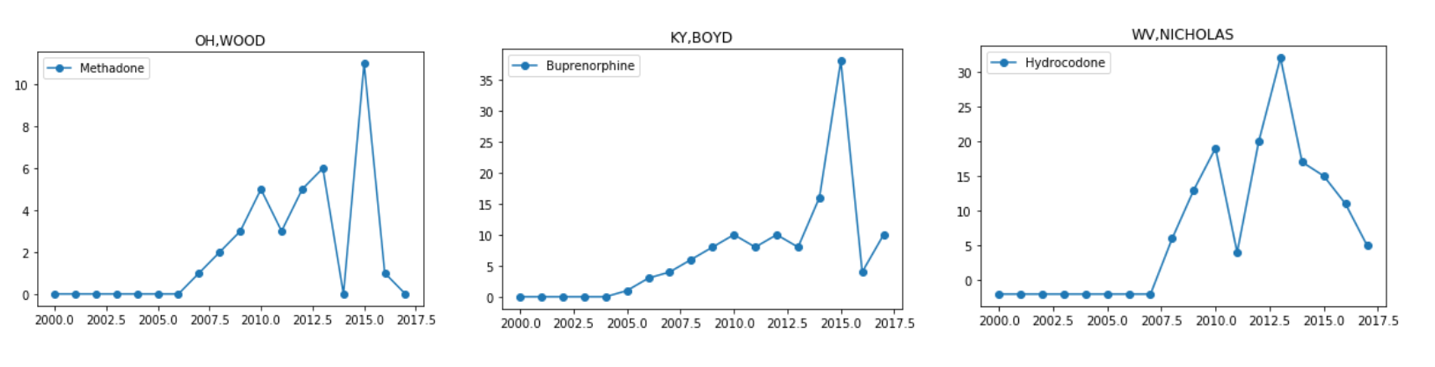
\includegraphics[width=1.0\linewidth]{OpioidCrisis/figures/prob1b.png} 
	\caption{Reversed simulation results in \textbf{Task} I.} 
	\label{fig:prob1b}  
\end{figure}

Secondly, we compute the total reported quantity of heroin and synthetic opioid between 2010 and 2017 and visualize the distribution(Figure \ref{fig:prob1a}). We observe that if the reported quantity of a specific drug is more than 200 and it kept increasing for more than 4 years, then the quantity tends to explode. Hence, the government should have specific concern on the counties that reach the drug identification threshold mentioned above.\\

\begin{figure}[h]
	\centering  
	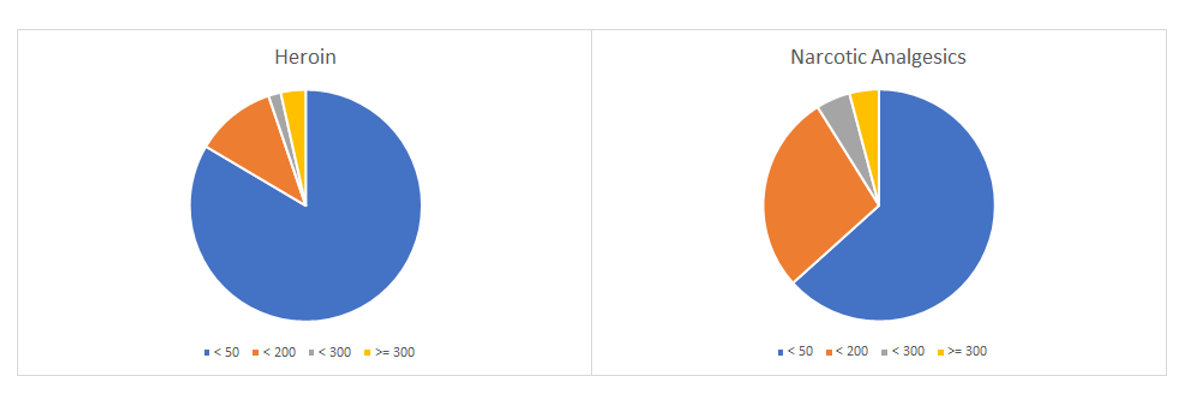
\includegraphics[width=1.0\linewidth]{OpioidCrisis/figures/prob1a.png} 
	\caption{Distribution of heroin and synthetic opioid reports quantity} 
	\label{fig:prob1a}  
\end{figure}

Thirdly, we simulate the reported quantity in 30 years for each specific drug. In our simulation, some of them tend to spread in some areas. The estimation of when and where they will reach the drug identification threshold levels are shown in Table \ref{tab:prob2}.

\renewcommand{\baselinestretch}{1.2}
\vspace{8pt}
\begin{table}[h]
\begin{center}
\setlength{\tabcolsep}{6mm}{
\begin{tabular}{|c|c|c|}
\hline
\textbf{Drug Name}& \textbf{County}& \textbf{Year}\\
\hline
\small{Buprenorphine}& \small{OH,HAMILTON}& \small{2018}\\
\hline
\small{Buprenorphine}& \small{PA,PHILADELPHIA}& \small{2019}\\
\hline
\small{Fentanyl}& \small{KY,BOONE}& \small{2014}\\
\hline
\small{Fentanyl}& \small{KY,CAMPBELL}& \small{2011}\\
\hline
\small{Fentanyl}& \small{PA,ALLEGHENY}& \small{2011}\\
\hline
\small{Fentanyl}& \small{PA,BEAVER}& \small{2019}\\
\hline
\small{Fentanyl}& \small{PA,MIFFLIN}& \small{2029}\\
\hline
\small{Fentanyl}& \small{PA,YORK}& \small{2011}\\
\hline
\small{Morphine}& \small{PA,PHILADELPHIA}& \small{2024}\\
\hline
\small{Oxycodone}& \small{OH,HAMILTON}& \small{2025}\\
\hline
\small{Oxycodone}& \small{OH,LAKE}& \small{2016}\\
\hline
\small{Oxycodone}& \small{OH,SUMMIT}& \small{2027}\\
\hline
\small{Oxycodone}& \small{OH,PHILADELPHIA}& \small{2010}\\
\hline
\small{Tramadol}& \small{OH,HAMILTON}& \small{2020}\\
\hline
\small{Tramadol}& \small{OH,MIAMI}& \small{2025}\\
\hline
\small{Tramadol}& \small{OH,MONTGOMERY}& \small{2021}\\
\hline
\small{Tramadol}& \small{PA,PHILADELPHIA}& \small{2016}\\
\hline
\end{tabular}}
\caption{Breakouts prediction of opioids in the future}
\label{tab:prob2}
\end{center}
\end{table}
\renewcommand{\baselinestretch}{1.0}


%% === 6.2 Results of D-OCEAN === %%

\begin{figure}[h]
	\centering  
	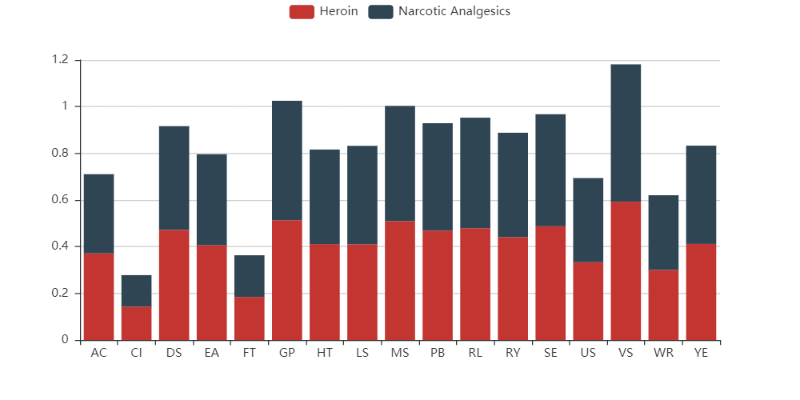
\includegraphics[width=1.0\linewidth]{OpioidCrisis/figures/Pearson.png} 
	\caption{Pearson correlation coefficients: demographic features - report quantity.(The meaning of the abbreviations on the axis can be found in Appendix\ref{tab:append}.)} 
	\label{fig:Pearson}  
\end{figure}

\begin{figure}[h]
	\centering  
	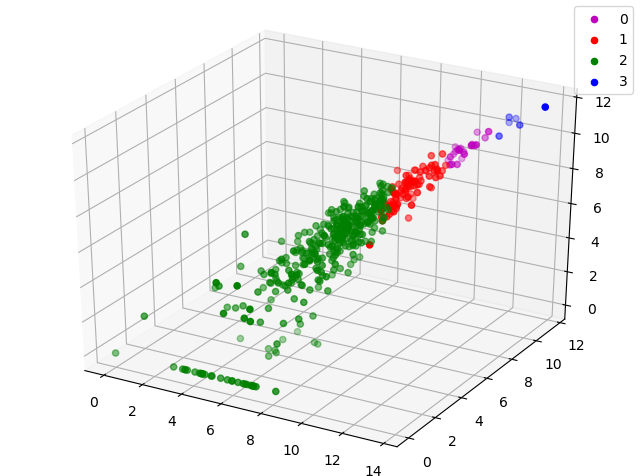
\includegraphics[width=0.8\linewidth]{OpioidCrisis/figures/kmeans.png} 
	\caption{An example of K-means results.} 
	\label{fig:kmeans}  
\end{figure}

\subsection{\textbf{Task II} Results of \texttt{D-OCEAN}}
In this task, we first compute the Pearson correlation coefficient between the reported quantity of the drugs and the factors in the provided U.S. Census socio-economic data. We observe that some factors like veteran, disability, and marital status are closely related to the reported quantity. The Pearson correlation coefficients are shown in Figure \ref{fig:Pearson}.\\

We choose the factors with the correlation coefficient higher than the threshold 0.85 as the main factors, then we apply K-means algorithm to cluster the counties into 4 classes and apply the corresponding score to them as described in Section \ref{sec4.4}. Figure, \ref{fig:kmeans} shows an example of cluster result.\\

\begin{figure}[h]
	\centering  
	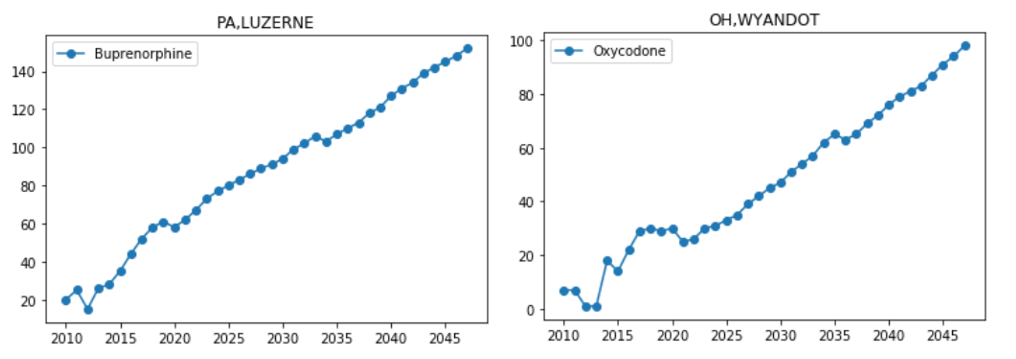
\includegraphics[width=1.0\linewidth]{OpioidCrisis/figures/prob21.png} 
	\caption{Simulation results: Buprenorphine in PA,LUZERNE and Oxycodone in OH,WYANDOT using \texttt{OCEAN} model.} 
	\label{fig:prob2a}  
\end{figure}

\begin{figure}[h]
	\centering  
	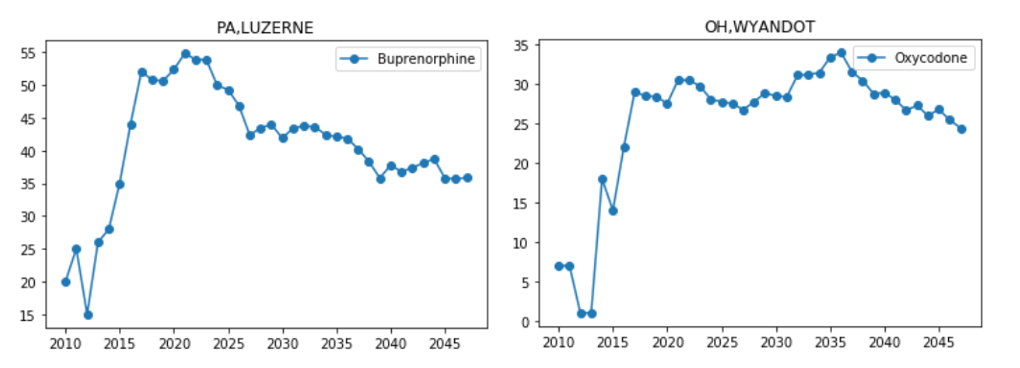
\includegraphics[width=1.0\linewidth]{OpioidCrisis/figures/prob22.png} 
	\caption{Simulated results of Buprenorphine in PA,LUZERNE and Oxycodone in OH,WYANDOT using \texttt{D-OCEAN} model.} 
	\label{fig:prob2b}  
\end{figure}

From Figure \ref{fig:kmeans}, we can clearly see that the counties are separated well. And although in most cases, the result of K-means algorithm may be different when the initial centers change, in our experiment, we run the K-means algorithm for several times but the result are the same. These indicate that the features we selected are distinguishable. After clustering, we compute the mean drug reported quantity inside each class, the results are shown in Table \ref{tab:prob2_res}. We can see that the mean reported quantity varies greatly from one class to another, this further proof that the feature we selected are closely related to the reported quantity. Hence the use factor $a^{(c_n)}$ and trends-in-use factor $b^{(c_n)}$ can well characterize the use and trends-in-use pattern of a county. We then modify our model as described in Section \ref{sec4.4} using the computed factors $a^{(c_n)}$ and $b^{(c_n)}$ to include some important factors in the dataset provided in \textbf{Task II}. Then we run our cellular automata again to obtain new simulated results. Some examples are showed in Figure \ref{fig:prob2a} \ref{fig:prob2b}.\\


\renewcommand{\baselinestretch}{1.2}
\vspace{8pt}
\begin{table}[h]
\begin{center}
\setlength{\tabcolsep}{6mm}{
\begin{tabular}{|c|c|}
\hline
\textbf{Class}& \textbf{Mean quantity of the class}\\
\hline
\small{0}& \small{2284.7619}\\
\hline
\small{1}& \small{965.4268}\\
\hline
\small{2}& \small{290.9261}\\
\hline
\small{3}& \small{11762.6666}\\
\hline
\end{tabular}}
\caption{Mean total drug reported quantity inside the cluster class.}
\label{tab:prob2_res}
\end{center}
\end{table}
\renewcommand{\baselinestretch}{1.0}


It's obvious that the growth of the drug reported quantity in some counties slowed down. This illustrates that our \texttt{D-OCEAN} model performs better when take some important socio-economic factors into account. 

\subsection{\textbf{Task III.} Crisis Respond Strategies}
As mentioned in Section \ref{section 5.2}, we conduct our experiment using several different vaules for parameters $\beta, a^{(c_n)}, b^{(c_n)}$, and test the effectiveness by computing the number of counties awash in drugs under different parameter setting. The results are shown in \textbf{Table} \ref{tab:prob3_res}.\\

\renewcommand{\baselinestretch}{1.2}
\vspace{8pt}
\begin{table}[h]
\begin{center}
\setlength{\tabcolsep}{6mm}{
\begin{tabular}{|c|c|c|c|}
\hline
\textbf{$\beta$}&\textbf{Upperbound of $a^{(c_n)}$}&\textbf{Lowerbound of $b^{(c_n)}$}& \textbf{$\delta$}\\
\hline
\small{$\beta\sim \mathcal{N}(0.3,0.1)$}& 1.0& 1.0&\small{1.0}\\
\hline
\small{$\beta\sim \mathcal{N}(0.1,0.1)$}& 1.0& 1.0&\small{1.4}\\
\hline
\small{$\beta\sim \mathcal{N}(0.3,0.1)$}& 1.0& 0.7&\small{5.3}\\
\hline
\small{$\beta\sim \mathcal{N}(0.3,0.1)$}& 0.7& 1.0&\small{3.2}\\
\hline
\small{$\beta\sim \mathcal{N}(0.3,0.1)$}& 0.7& 0.7&\small{10.7}\\
\hline
\end{tabular}}
\caption{Quantity results of the effectiveness of strategies in \textbf{Task III}. (Ratio $\delta$ - higher is better - is defined in Section \ref{section 5.2}.)}
\label{tab:prob3_res}
\end{center}
\end{table}
\renewcommand{\baselinestretch}{1.0}


We can see that a small $\beta$ and a small upperbound of $a^{(c_n)},b^{(c_n)}$ can effectively tackle the opioid crisis, and in our experiment, we found that when $a^{(c_n)} < 0.75$ and $b^{(c_n)} < 0.85$, the proposed strategy is very effective to counter the opioid crisis. 


%% === 7. Experiment Analysis === %%
\vspace{8pt}
\section{Further Analysis}

%% === 7.1 Effectiveness Analysis === %%
\subsection{Effectiveness Analysis}
In order to evaluate the effectiveness of our model, we use the provide data in \textbf{Task I} between year 2010 and 2013 to compute some parameters for our model, and then we run our cellular automata to simulate the reported quantity of each drug in each county between year 2014 and 2017, then we compare the simulated results with the given data. If the trend of reported quantity of a specific drug in a county in a specific year are same in the simulated results and the given data(e.g., the quantity increase in both the simulated results and the given data in that year), we consider our the prediction is right in that year. In this way, we compute our prediction accuracy and the results are shown in Figure \ref{fig:acc}. We can see that our prediction accuracy is high which confirms the effectiveness of our model.

\begin{figure}[h]
	\centering  
	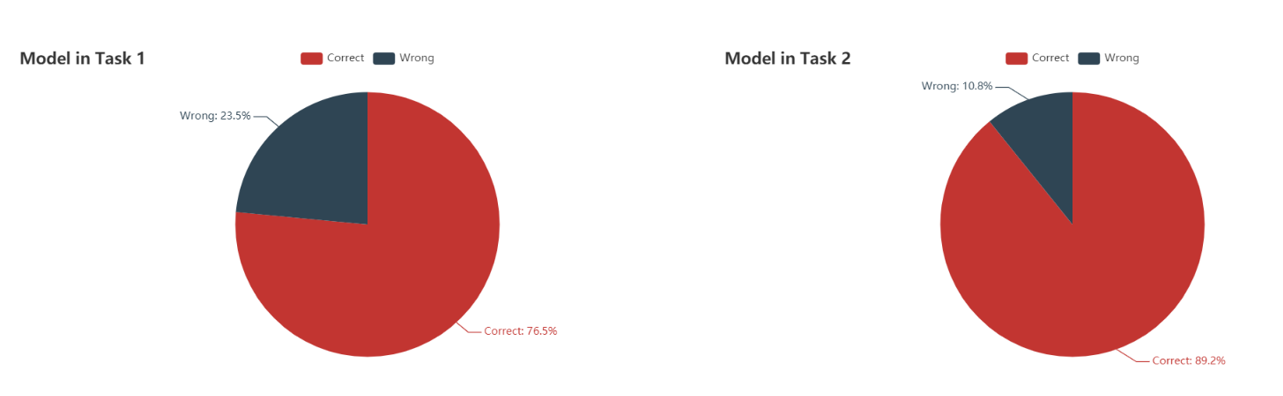
\includegraphics[width=1.0\linewidth]{OpioidCrisis/figures/acc.png} 
	\caption{The prediction accuracy of our model.} 
	\label{fig:acc}  
\end{figure}

%% === 7.2 Sensitivity Analysis === %%
\subsection{Sensitivity Analysis}
We test the sensitivity by adjusting different parameters in the model. Firstly, as shown in results of \textbf{Task II}, our K-means algorithm reach same result when different initial centers are selected, this indicates that K-means algorithm is not sensitive to the initial centers using the features we selected. Secondly, we decrease the threshold of the Pearson correlation coefficient, in this way, there are more socio-economic factors that we should consider, but the influence on the result is so slightly that it can be neglect. Finally, we apply different values to other parameters in our model, then we found that our model is sensitive to the $\alpha, \beta$(incremental parameters), $k_{in}, k_{ex}$ (weights of intrinsic and extrinsic opioid growth quantity) and $\lambda$(growth factor of estimate incremental). We argue that in real world, the drug reported quantity increasing pattern is also sensitive to those factors.


%% === 8. Strengths and Weaknesses === %%
\section{Strengths and Weaknesses}

%% === 8.1 Strengths === %%
\subsection{Strengths}

\begin{itemize}
  \item \textbf{High Scalability:} Although designed in detail, our model actually presents some macro discussions. Government can put our strategies into practice from many aspects in similar situations. We only introduce some typical features of drug incidents, and try to simulate the changing process by computers. As we do not fit problems into specific models, our models take effect in most cases.
  \item \textbf{High Reliability:} High reliability is ensured by the following two techniques.
  \begin{itemize}
      \item \textit{\textbf{Bilateral Analysis:}} In D-OCEAN, our results have been \textbf{reversely verified} to ensure reliability. We first conduct correlation calculation to screen out highly correlated demographic features. Luckily, results of this step are verified by the fact that points are separated well by K-means algorithm.
      \item \textit{\textbf{Mass Data Analysis:}} We used large amounts of data in real dataset in latest years. In \textbf{Task I}, we deal with data with 63 kinds of opioids and 24062 drug reports. In \textbf{Task II}, 17 demographic features and 198 valid subordinate classes are involved to solve our problem. Strong data support is the guarantee of our reliability.
  \end{itemize} 
  \item \textbf{Low Cost:} Although the validity of our model is based on a large architecture, each part of the system is not of high complexity. \textbf{Cosine} and \textbf{Pearson} correlation analysis are both efficient similarity measurement methods. \textbf{K-means} algorithm only has linear time complexity. Core steps in our models are all economical but effective.
  
\end{itemize}

%% === 8.1 Weaknesses === %%
\subsection{Weaknesses}

\begin{itemize}
  \item \textbf{Lack of Old Data}: The data we get are not very comprehensive, to some extent, affecting the accuracy of our results on relevant situations.
  \begin{itemize}
      \item \textit{\textbf{Incomplete Year:}} Data we collect are from latest years, but many opioid epidemics begin extremely early before 2000. Our study lacks consideration of the early conditions, which means that our estimate might not be so accurate for in early years.
      \item \textit{No Other States:} Limited by the data given, we have difficulties to have a clear clue about other states. This prevent us from depicting a overall opioid profile of the U.S.
  \end{itemize}
  \item \textbf{Relatively Crude Consideration:} Due to time constraints, we are unable to draw a splendid picture of opioid cases without some slightly influencing factors (e.g. the production of certain opioid-related raw materials). Nevertheless, we considered the main factors in general cases and proved the validity of our model. Once these tiny factors are considered in detail, our model becomes more complete.
  \item \textbf{Lack Methods Comparison}: Due to time constraints, we only adapt the most advanced model as far as we known. There may exist other more desirable models to explore in the future.
\end{itemize}

\clearpage
\renewcommand{\baselinestretch}{2}
\section{Memo for Chief Administrator}
\setlength{\baselineskip}{14pt}
\textsf{Dear Sir:}

\textsf{As the opioid crisis intensified, we are beginning to realize the seriousness of the problem and all trying to find causes of this catastrophe. Upon hearing your program is trying to find associated information with complete database, our teams are honored to engage in investigating drug cases evolution and characterization. We have been working with painstaking efforts so as to make an accurate prediction, and we do have some outcome by researching day and night these days, which we hope can offer some important insights for you.}

\textsf{Inspired by the performance of cellular automaton in research of complex socio-economic systems, we employed it for simulating the evolution patterns of opioids. Taking account of demographic heterogeneity in each state, we enhanced our model by introducing some socio-economic factors. Finally, corresponding solutions were put forward, according to the analysis of our models. Our insights are listed as follows.}

\textsf{On one hand, the drugs might spread from one county to another. As the experimental results show, we find that geography is an important factor that affects the level of drug detection. When the drug detection level in a county rises, so does the detection level in the surrounding counties. Therefore, we suggest that when the detection level of some counties is high, the government need to strengthen the supervision on these counties to impede the spread of drug use.}

\textsf{On the other hand, we also analyzed the correlation between the county's socio-economic characteristics and the level of drug detection, and we found that they were highly relevant in some indicators like number of veterans, disabled. Our analysis indicates that the number of vulnerable groups in society such as widows, persons with disabilities, veterans, etc. was highly correlated with the number of drug addicts. We believe that targeted assistance to such groups will enrich their daily lives and improve their well-being. We believe that in this way, the number of people who choose to use drugs among these groups will be greatly reduced.}

\textsf{In conclusion, we recommend the U.S. government to take following strategies to cope with this severe problem. Internally, medical institutions should try to limit the amount of narcotics used by special groups (such as the disabled and retired veterans) and improve the existing medical security system; local governments are supposed to raise their oversight of vulnerable audiences with high rates of opioid addiction. Externally, strengthen drug control in counties, where drugs reports have exceeded the alert level, and their nearby.}

\textsf{With our validation, we think these actions can truly improve the opioid epidemic situation and our sensitivity analysis can tell you the utility of each strategy. We firmly believe that our efforts will create a better medical and living environment for all!}

\noindent \textsf{Best regards,}

\noindent \textsf{Sincerely}
\clearpage
\renewcommand{\baselinestretch}{1.0}

\bibliographystyle{plainnat}
\bibliography{main}
\clearpage

\section*{\Large{Appendices}}

\subsection*{}
\begin{figure}[h]
  \small
  \centering
  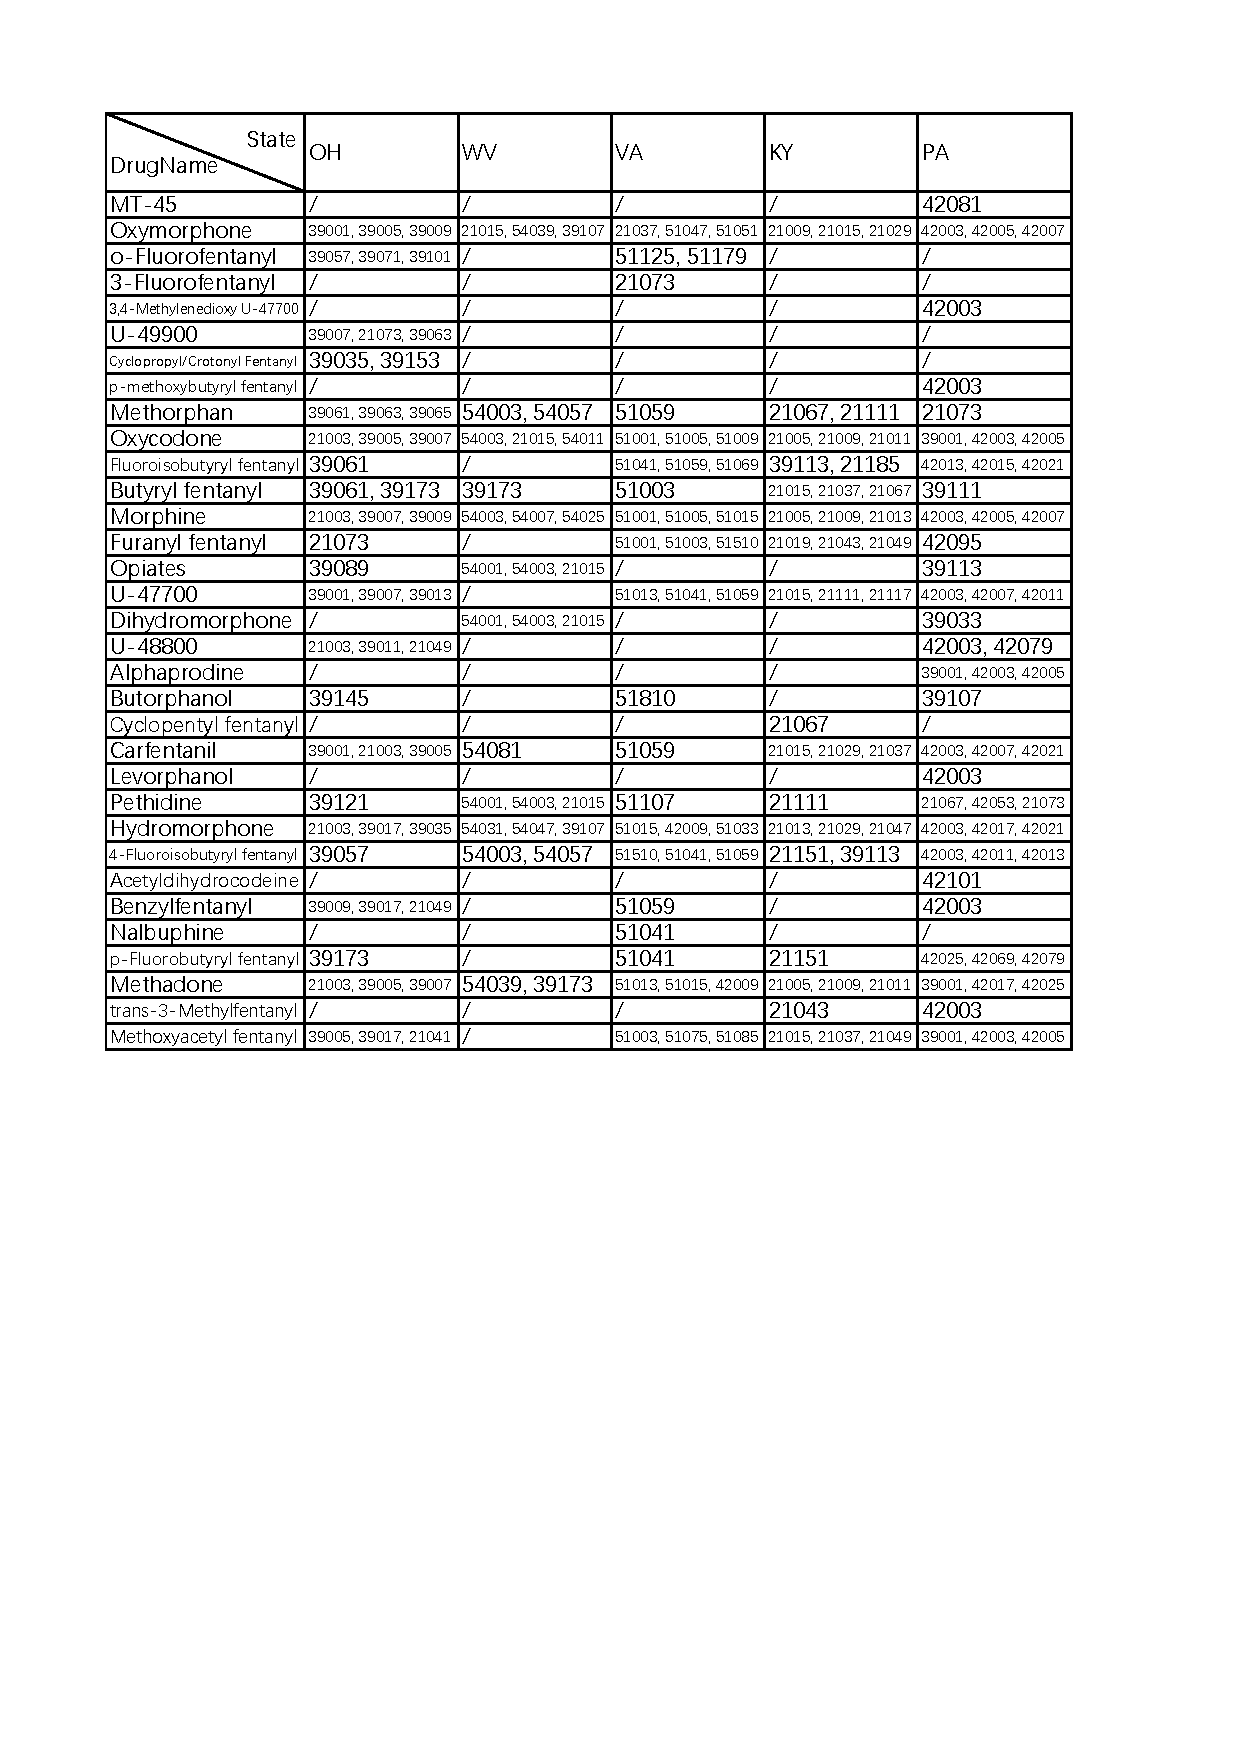
\includegraphics[width=18cm,height=27cm]{OpioidCrisis/figures/sheet1.pdf}
  \caption{Complete result for \textbf{Task I}, the county are expressed by FIPS.}
\end{figure}

\begin{figure}[h]
  \small
  \centering
  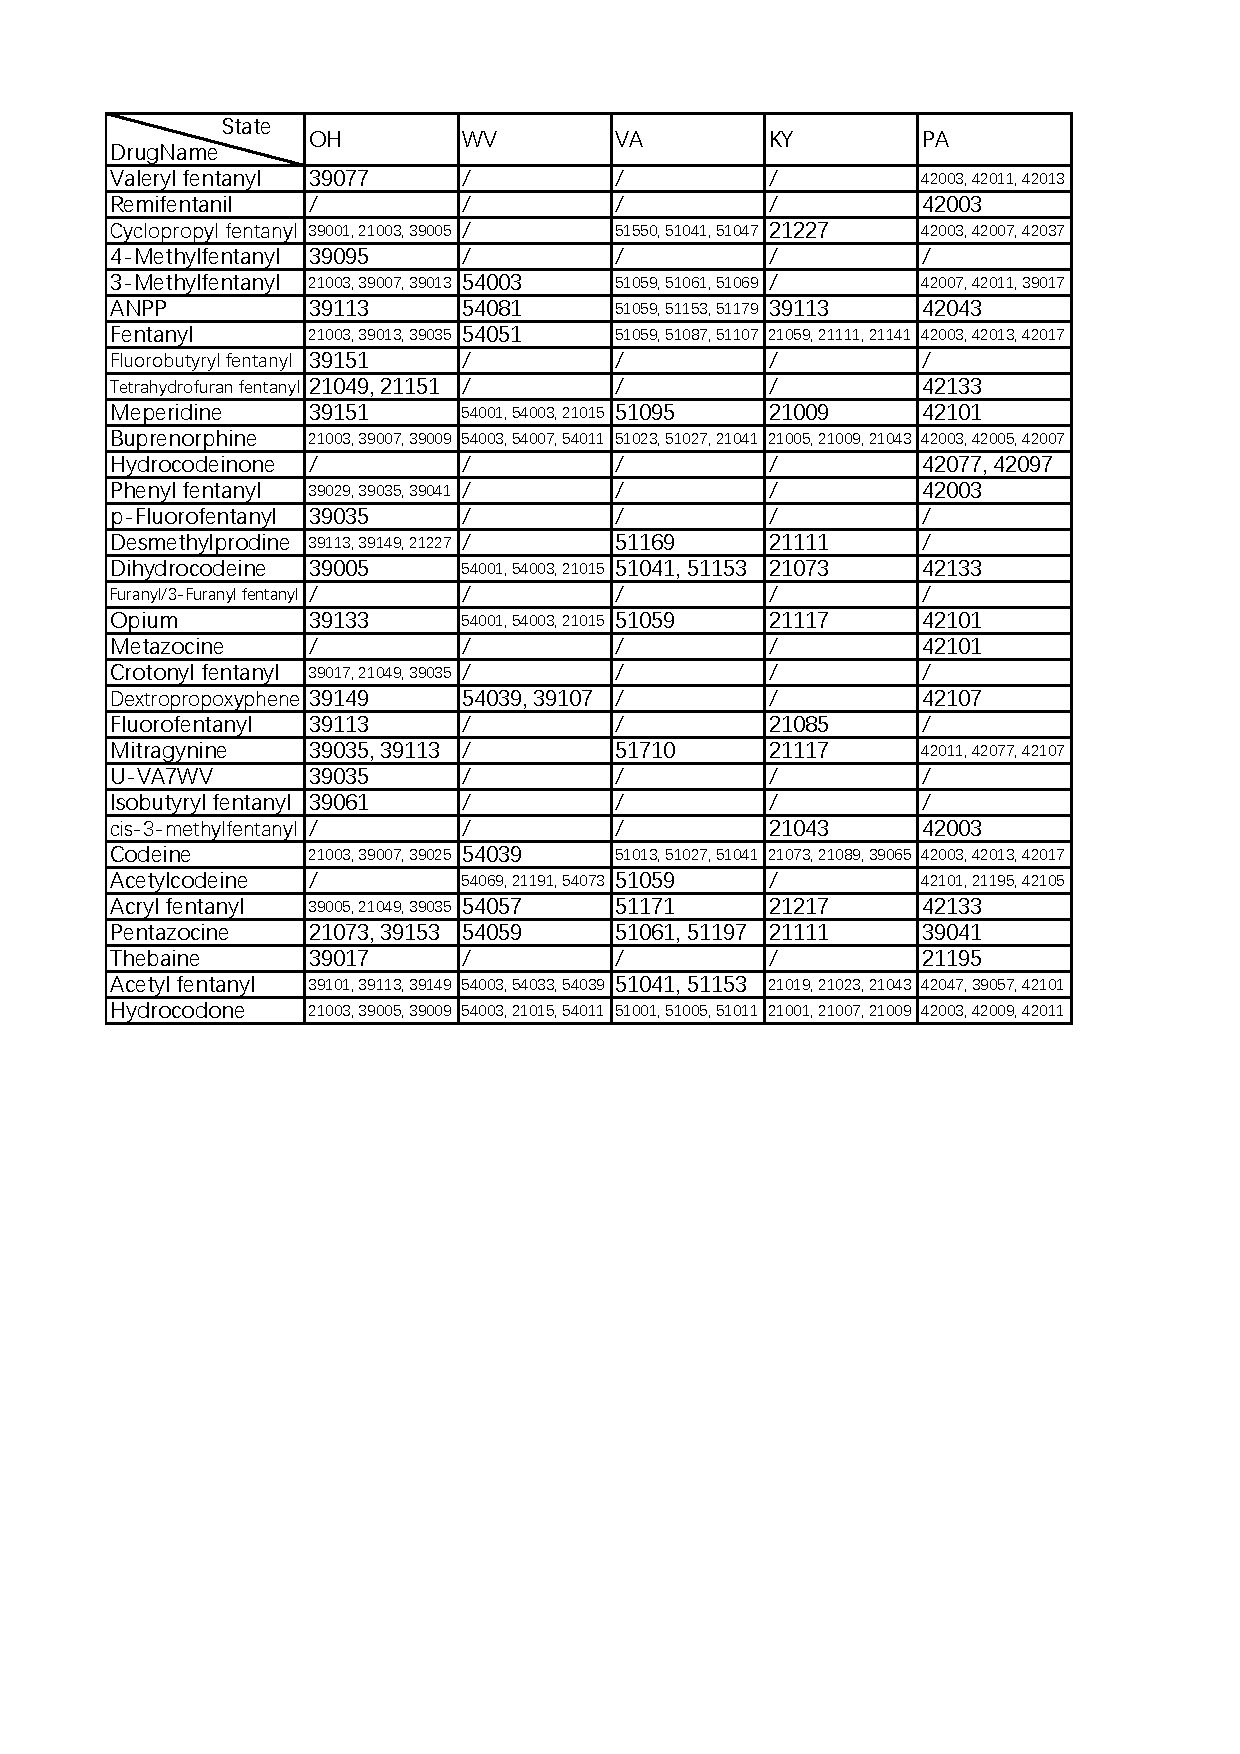
\includegraphics[width=18cm,height=27cm]{OpioidCrisis/figures/2.pdf}
  \caption{Complete result for \textbf{Task I}, the county are expressed by FIPS.}
\end{figure}

\subsection*{The meaning of the abbreviations on the axis.}
\renewcommand{\baselinestretch}{1.3}
\begin{table}[h]
\begin{center}
\setlength{\tabcolsep}{6mm}{
\begin{tabular}{|c|c|}
\hline
\textbf{Abbreviation}& \textbf{Category}\\
\hline
\small{AC}& \small{ANCESTRY}\\
\hline
\small{CI}& \small{COMPUTERS AND INTERNET USE}\\
\hline
\small{DS}& \small{DISABILITY STATUS OF}\\ 
 &\small{THE CIVILIAN NONINSTITUTIONALIZED POPULATION}\\
\hline
\small{EA}& \small{EDUCATIONAL ATTAINMENT}\\
\hline
\small{FT}& \small{FERTILIT}\\
\hline
\small{GP}& \small{GRANDPARENTS}\\
\hline
\small{HT}& \small{HOUSEHOLDS BY TYPE}\\
\hline
\small{LS}& \small{LANGUAGE SPOKEN AT HOME}\\
\hline
\small{MS}& \small{MARITAL STATUS}\\
\hline
\small{PB}& \small{PLACE OF BIRTH}\\
\hline
\small{RL}& \small{RELATIONSHIP}\\
\hline
\small{RY}& \small{RESIDENCE 1 YEAR AGO}\\
\hline
\small{SE}& \small{SCHOOL ENROLLMENT}\\
\hline
\small{US}& \small{U.S. CITIZENSHIP STATUS}\\
\hline
\small{VS}& \small{VETERAN STATUS}\\
\hline
\small{WR}& \small{WORLD REGION OF BIRTH OF FOREIGN BORN}\\
\hline
\small{YE}& \small{YEAR OF ENTRY}\\
\hline
\end{tabular}}
\caption{Explanation of abbreviated words of category}
\label{tab:append}
\end{center}
\end{table}
\renewcommand{\baselinestretch}{1.0}
\clearpage{}

\subsection*{Code}

\noindent Part I - \textbf{corrcompute.py}
\lstinputlisting[language=python]{./code/corrcompute.py}

\noindent Part I - \textbf{prob1.py}
\lstinputlisting[language=python]{./code/prob1.py}

\noindent Part II - \textbf{prob2.py}
\lstinputlisting[language=python]{./code/prob2.py}

\noindent Part II - \textbf{kmeans.py}
\lstinputlisting[language=python]{./code/kmeans.py}

\noindent Part III - \textbf{prob3.py}
\lstinputlisting[language=python]{./code/prob3.py}

\clearpage

\end{document}